\icode{N24L-MCC-SI-L2-261025-002}
\nceeID[4]{2024辽宁}{2}
“指尖转球”是花式篮球表演中常见的技巧。如图，当篮球在指尖上绕轴转动时，球面上 \(P\)、\(Q\) 两点做圆周运动的\paren[]

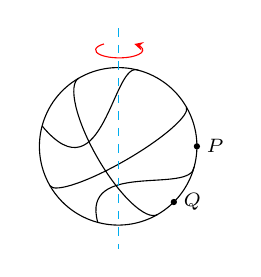
\begin{tikzpicture}[>=stealth,font=\scriptsize]
	\begin{scope}[rotate=30]
		\draw (0,0)coordinate(o) circle(1);
		\draw (0,-1) arc(270:90:.3 and 1) (-1,0) arc(-180:0:1 and .2);
		\draw (135:1)..controls(-.5,-.5)and(.5,1)..(45:1);
		\draw (-135:1)..controls(-.5,.1)and(.5,-1)..(-45:1);
	\end{scope}
	\draw[dashed,cyan] (0,1.5)--(0,-1.3);
	\draw[->,red] (-.18,1.3) arc(-230:50:.3 and .1);
	\fill (1,0)node[right]{\(P\)} circle(.04) (-45:1)node[right]{\(Q\)} circle(.04);
\end{tikzpicture}
\begin{choices}
	\item 半径相等
	\item 线速度大小相等
	\item 向心加速度大小相等
	\item 角速度大小相等
\end{choices}
\begin{answer}
	D\qquad 提示：\(P\)、\(Q\)同轴转运
\end{answer}